\chapter{搜索}

\section{人工智能}

\subsection{人工智能(Artificial Intelligence)}

我们称自己为智人,几千年来,我们一直试图了解我们是如何思考和行动的。\\

AI企图了解智能的实质,并生产出一种新的能以人类智能相似的方式做出反应的智能机器,该领域的研究包括机器人学、语言识别、图像识别、自然语言处理和专家系统等。\\

人类通过器官(眼、耳、鼻、口、皮肤)从外部环境进行感知,并做出一系列行为(说话、吃饭、移动、决策等)。\\

智能Agent通过传感器(麦克风、摄像头、陀螺仪、声呐等)从外部环境进行感知,从而进行规划、分类、预测等行为。\\

一个理性的Agent(Rational Agent)需要能进行理性的思考和行为,即在现有环境下,做出利益最大化的行为。\\

\subsection{AI的演变}

\subsubsection{基于逻辑的AI(Logic-Based AI)}

最初的人工智能是基于逻辑学的,数理逻辑的思想和方法一直在知识表示中发挥着重要作用。基于逻辑的AI的领域包括常识推理、溯因推理、归纳推理、计算逻辑、概率、规划、决策等。\\

建立在命题逻辑和谓词逻辑上的AI在九十年代前进入了寒冬,直到大量统计学方法引入之后才有了现在大热的机器学习。\\

\subsubsection{专家系统(Expert System)}

专家系统是一个智能计算机程序,其内部含有大量的某个领域专家水平的知识与经验,它根据系统中的知识与经验,进行推理和判断,模拟人类专家的决策过程,以便解决那些需要人类专家处理的复杂问题。\\

例如医疗诊断系统,它依靠病人的具体病况作为条件来分析,系统可根据病人的病情描述,在已有的知识与经验中,匹配最有可能的病症和治疗方案。\\

虽然专家系统看起来已经发展了很久,但是它并没有那么可靠。例如在实际的看病过程中,往往医生在除了问询之外,还有自己做推断的部分,目前的专家系统还没有办法做到对病人的病况了解的足够清晰。\\

其次专家系统的一大问题就是其潜在的风险性,包括无人驾驶汽车也有类似的问题。在发生问题之后,谁来背负责任呢?比如某患者采用了一个医疗专家系统,然后听从专家系统的指示,可结果病情却越来越重。\\

\subsubsection{机器学习(Machine Learning)}

机器学习是一门多领域交叉的学科,涉及概率论、统计学、逼近论、凸分析、算法复杂度理论等多门学科,专门研究计算机怎样模拟或实现人类的学习行为,以获取新的知识或技能,重新组织已有的知识结构使之不断改善自身的性能。\\

例如在自动驾驶中需要通过机器视觉不断看到周围的物体,然后通过机器学习来辨识出这些物体是什么(人、车、交通灯等)。学会辨识图片的过程需要输入大量的车辆的图片给机器学习,最后它就会知道这些图片代表的是车。

\begin{figure}[H]
    \centering
    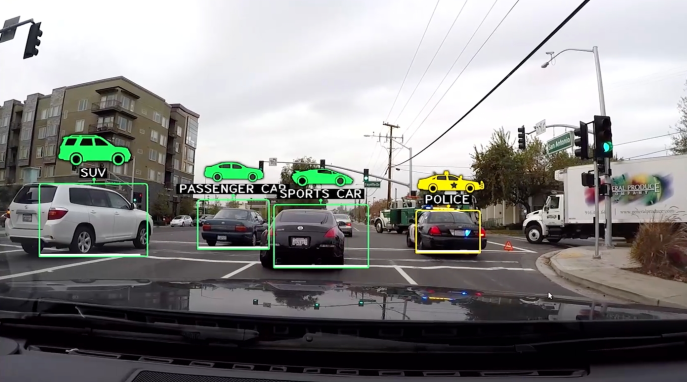
\includegraphics{img/C1/1-1/1.png}
    \caption{自动驾驶}
\end{figure}

机器学习最重要的是预测,比如通过大量的图片学会什么是车后,再来一张没有见过的车辆的图片,我们希望机器可以做出正确的判断。因此机器学习包含训练和预测两个部分,并且要保证一定的正确率。\\

\subsubsection{深度学习(Deep Learning)}

深度学习是一种深层次的学习,以教儿童认字为例,按照字从简单到复杂的顺序,让儿童反复看每个字的各种写法,并自己临摹。看得多了,自然就记住了。下次再见到同一个字,就很容易能认出来。认字时,一定是儿童的大脑在接受许多遍相似图像的刺激后,为每个字总结出了某种规律性的东西,下次大脑再看到符合这种规律的图案,就知道是什么字了。\\

计算机在识别时,也要先把每一个图案反复看很多很多遍,然后在总结出一个规律,以后计算机再看到类似的图案,只要符合之前总结的规律,计算机就能知道这是什么图案。用专业的术语来说,计算机用来学习的、反复看的图片叫训练数据集。

\begin{figure}[H]
    \centering
    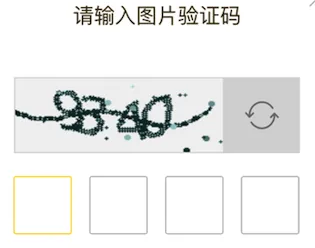
\includegraphics{img/C1/1-1/2.png}
    \caption{验证码}
\end{figure}

深度学习与机器学习的主要区别是在于性能。当数据量很少的时候,深度学习的性能并不好,因为深度学习算法需要大量数据才能很好理解其中蕴含的模式。因此深度学习算法严重依赖高端机,而传统的机器学习算法在低端机上就能运行。深度学习需要GPU(Graphics Processing Unit)进行大量的矩阵乘法运算。

\newpage

\section{状态空间}

\subsection{智能Agent}

智能Agent的设计取决于一系列因素:

\begin{itemize}
    \item 环境:静态(static)、动态(dynamic)
    \item 表示方案(representation scheme):状态(state)、特征(feature)、关系(relation)
    \item 可观察性(observability):完全可观察、部分可观察
    \item 参数类型:离散(discrete)、连续(continuous)
    \item 不确定性(uncertainty):确定性(deterministic)、随机性(stochastic)
    \item 学习:知识是给定的(已知的),知识是学来的(未知的)
    \item Agent数量:单Agent、多Agent
\end{itemize}

\vspace{0.5cm}

\subsection{状态空间(State Space)}

假设有两个有灰尘的房间A和B,吸尘器一开始位于房间A,吸尘器只能进行左移、右移和吸尘三个操作,最终的目标是将两个房间内的灰尘清扫完毕。\\

因此根据房间有无灰尘和吸尘器的位置,一共存在8种状态。

\begin{figure}[H]
    \centering
    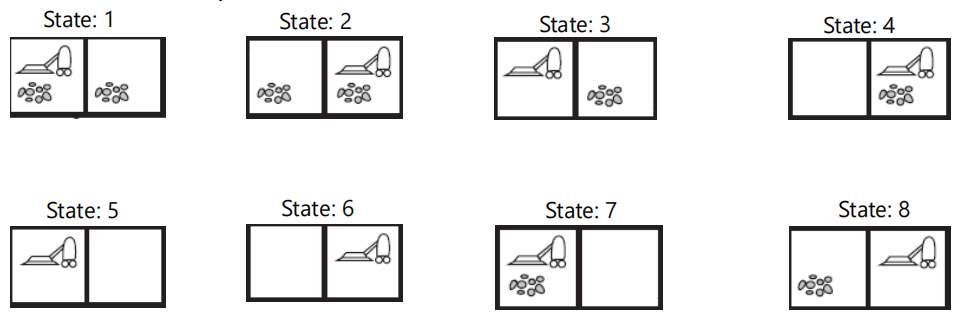
\includegraphics[scale=0.7]{img/C1/1-2/1.png}
\end{figure}

\begin{table}[H]
    \centering
    \setlength{\tabcolsep}{5mm}{
        \begin{tabular}{|c|c|c|c|}
            \hline
            \textbf{状态} & \textbf{房间A} & \textbf{房间B} & \textbf{吸尘器位置} \\
            \hline
            1             & 脏             & 脏             & A                   \\
            \hline
            2             & 脏             & 脏             & B                   \\
            \hline
            3             & 干净           & 脏             & A                   \\
            \hline
            4             & 干净           & 脏             & B                   \\
            \hline
            5             & 干净           & 干净           & A                   \\
            \hline
            6             & 干净           & 干净           & B                   \\
            \hline
            7             & 脏             & 干净           & A                   \\
            \hline
            8             & 脏             & 干净           & B                   \\
            \hline
        \end{tabular}
    }
\end{table}

假设以状态6作为目标状态(goal state),可以得到状态空间图:

\begin{figure}[H]
    \centering
    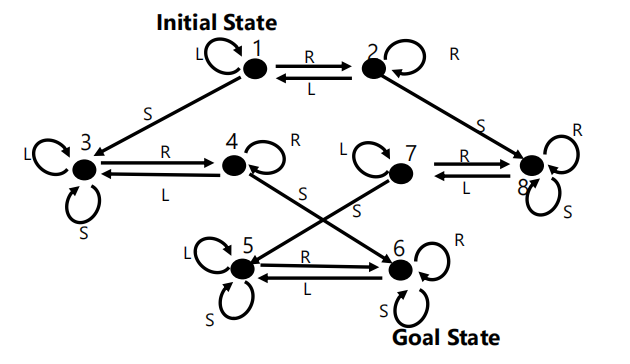
\includegraphics{img/C1/1-2/2.png}
\end{figure}

提取问题中的特征:

\begin{itemize}
    \item $ status = \{clean, dirty\} $
    \item $ location = \{A, B\} $
    \item $ actions = \{suck, left, right\} $
\end{itemize}

吸尘器的处理过程可以表示为:

\begin{algorithm}[H]
    \caption{VacuumCleaner}
    \begin{algorithmic}[1]
        \Procedure{VacuumCleaner}{status, location}
        \If {status = dirty}
        \State return suck
        \EndIf

        \If {location = A and status = clean}
        \State return right
        \EndIf

        \If {location = B and status = clean}
        \State return left
        \EndIf
        \EndProcedure
    \end{algorithmic}
\end{algorithm}

\vspace{0.5cm}

\subsection{性能评估(Performance Measure)}

算法的性能评估包含以下几个方面:

\begin{itemize}
    \item 完备性(completeness)
          \begin{itemize}
              \item 完备(Complete):算法可以到达目标状态
              \item 不完备(incomplete):算法无法到达目标状态
          \end{itemize}
    \item 正确性
    \item 最优性(optimality):算法以最优解(最小代价)找到到达目标状态的路径
    \item 时间复杂度(time complexity):求解所需的时间
    \item 空间复杂度(space complexity):求解所需的存储空间
\end{itemize}

\newpage

\section{盲目搜索/无信息搜索}

\subsection{盲目搜索/无信息搜索(Uninformed Search)}

当需要采取的正确行动不是显而易见时,Agent就需要提前规划,考虑能够通往目标状态的一系列行动,Agent所进行的计算过程被称为搜索。\\

对于一个问题,首先需要确定它的初始状态(initial state)和目标状态,其次需要对问题进行建模(modeling)。一个问题的建模包括6个部分:

\begin{enumerate}
    \item 状态集合
    \item 初始状态
    \item 行为集合$ Actions(s) $:在状态$ s $时所有合法的行为集合
    \item 状态转移$ Result(s, a) $:返回在状态$ s $时执行行为$ a $后的状态
    \item 目标状态:使用$ IsGoal(s) $来判断状态$ s $是否为目标状态
    \item 行为代价函数(Action Cost Function):在某个状态执行某个行为所需的代价,使用$ ActionCost(s, a, s') $表示在状态$ s $执行行为$ a $到达状态$ s' $所需的代价
\end{enumerate}

在八数码(8-puzzle)问题中,在一个3*3的方格中,有数字1~8和一个空白,最终需要将数字依次排列,使空白位于最后的位置。\\

八数码问题一共存在$ 9! = 362880 $种状态,其中初始状态为任意一种摆放布局,目标状态为依次排列的布局。

\begin{figure}[H]
    \centering
    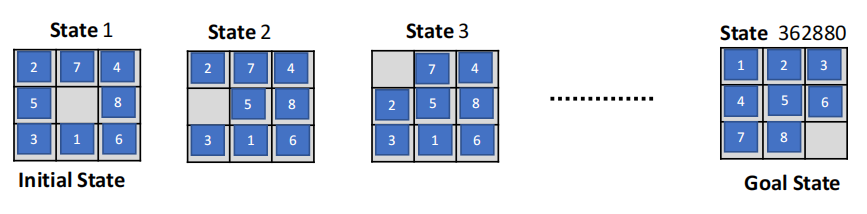
\includegraphics[scale=0.8]{img/C1/1-3/1.png}
\end{figure}

行为包括可以将空白进行上移(U)、下移(D)、左移(L)、右移(R),每次移动的代价可以认为都为1,例如对初始状态中的空白进行左移,其状态转移可表示为$ s_2 = Result(s_1, L) $。\\

在罗马尼亚地图(Romania map)中,例如初始位置位于Arad,最终想要到达Bucharest。问题的状态为所有的城市,每次行动的代价为城市见的距离。

\begin{figure}[H]
    \centering
    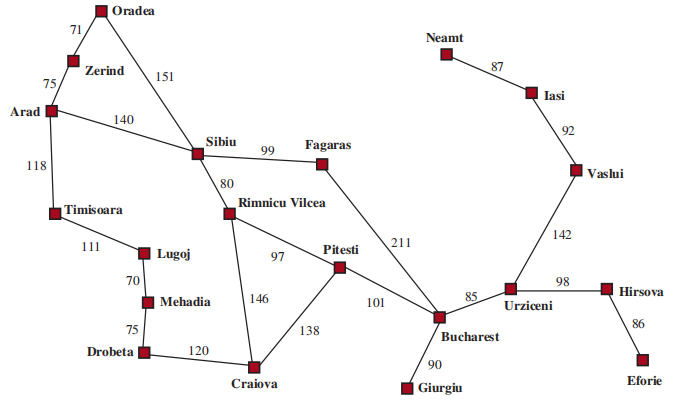
\includegraphics{img/C1/1-3/2.png}
    \caption{罗马尼亚地图}
\end{figure}

\vspace{0.5cm}

\subsection{搜索树(Search Tree)}

